% * Preamble
\documentclass[xcolor=dvipsnames]{beamer}
\synctex=1
\usepackage[UTF8,scheme=plain]{ctex}
\usepackage{hyperref}
\usepackage{lmodern}
\usepackage{mathrsfs}
\usepackage{graphicx}
\usepackage[export]{adjustbox}
\usepackage{comment}
\usepackage{mathtools}
\mathtoolsset{showonlyrefs}
\usetheme{Madrid}
\usecolortheme{seahorse}
\usecolortheme{rose}
\usefonttheme{serif}
\usefonttheme{structurebold}
\setbeamerfont{title}{shape=\itshape,family=\rmfamily}
\setbeamercolor{title}{fg=red!80!black,bg=red!20!white}
% * Top matter
\title[Critical Superprocesses]{Limit theorems for a class of critical superprocesses with stable branching}
\author[Z. Sun]{
{\bf \Large Zhenyao Sun}\inst{1} \\
}
\institute[PKU]{
  Based on a joint work with {\bf Yan-Xia Ren}\inst{1} and {\bf Renming Song}\inst{2}\\
  \inst{1} Peking University \\
  \inst{2} University of Illinois at Urbana-Champaign\\
}
\date[UIBE, June, 2019]{
  University of International Business and Economics\\ 
  June, 2019}
\begin{document}

% * Title page
\begin{frame}
  \titlepage
\end{frame}
% * Outline
\begin{frame}
  \frametitle{Outline}
  \tableofcontents
\end{frame}

% * Background
\section{Background}
% ** Kolmogorov's result
\subsection{Kolmogorov's result}
\begin{frame}{Background/Kolmogorov's result}
  \begin{theorem}[Kesten, Ney and Spitzer (1966)]
Let $(Z_n)_{n\in \mathbb N}$ be a critical Galton-Watson process with offspring variance $\sigma^2 \in (0,\infty)$. 
Then
\begin{align}
n P(Z_n > 0) \xrightarrow[n\to \infty]{} \frac{2}{\sigma^2}.
\end{align}
\end{theorem}
\begin{itemize}
\item
Kolmogorov (1938) obtained the above Theorem under a three moment condition.
\end{itemize}
\end{frame}

% ** Yaglom's result
\subsection{Yaglom's result}
\begin{frame}{Background/Yaglom's result}
\begin{theorem}[Kesten, Ney and Spitzer (1966)]
Let $(Z_n)_{n\in \mathbb N}$ be a critical Galton-Watson process with offspring variance $\sigma^2 \in (0,\infty)$.
Then 
\begin{align}
  \left\{ \frac{Z_n}{n}; P(\cdot | Z_n > 0) \right\} 
\xrightarrow[n\to \infty]{d} \frac{\sigma^2}{2} {\color{red} \mathbf e},
\end{align}
where {\color{red} $\mathbf e$} is an exponential random variable with mean $1$.
\end{theorem}
\begin{itemize}
\item
Yaglom (1947) obtained the above Theorem under a stronger condition.
\end{itemize}
\end{frame}

% ** Slack's result
\subsection{Slack's result}
\begin{frame}{Background/Slack's result}
\begin{theorem}[Slack (1968)]
	Let $(Z_n)_{n\geq 0}$ be a critical Galton-Watson process with offspring generating function
$
	f(s)
	= s + (1-s)^{\alpha} l(1-s)
$
  where $\alpha \in (1,2]$ and $l$ is a slowly varing function at $0$.
  Then
$
	P(Z_n > 0) = n^{-1/(\alpha-1)} L(n)
$ 
where $L$ is slowly varying at $\infty$;
 and
\[
  \big\{ P(Z_n > 0) Z_n; P(\cdot | Z_n > 0)\big\}
	\xrightarrow[n\to \infty]{d} {\color{red}\mathbf z^{(\alpha-1)} },
\]
	where {\color{red} $\mathbf z^{(\alpha-1)}$} is a positive random variable with Laplace transform
\[
	E[e^{- u {\color{red} \mathbf z^{(\alpha-1)}} } ]
	= 1 - (1+ u^{-(\alpha-1)})^{-1/(\alpha-1)},
	\quad u \geq 0.
\]
\end{theorem}
\begin{itemize}
\item
  Zolotarev (1957) obtained the above Theorem under a stronger condition.
\end{itemize}
\end{frame}

\begin{frame}
\begin{table}[] 
\resizebox{\textwidth}{!}{%
\begin{tabular}{|l|l|l|l|}
\hline
& $\alpha = 2$: Analytical 
& $\alpha = 2$: Probabilistic 
& $\alpha \in (1,2)$ 
\\ \hline
\begin{tabular}[c]{@{}l@{}} Galton-Watson \\ (GW) processes \end{tabular} 
& \begin{tabular}[c]{@{}l@{}} Kolmogorov (1938)\\ Yaglom (1947)\\ Kesten, Ney \\ and Spitzer (1966) \end{tabular} 
& \begin{tabular}[c]{@{}l@{}} Lyons, Pemantle \\ and Peres (1995)\\ Geiger (1999) \\ Geiger (2000)\\ {\color{red} Ren, Song} \\ {\color{red} and Sun (2018)}\end{tabular} 
& \begin{tabular}[c]{@{}l@{}} Zolotarev (1957)\\ Slack (1968)\end{tabular} 
\\ \hline
\begin{tabular}[c]{@{}l@{}} Multitype GW \end{tabular} 
& \begin{tabular}[c]{@{}l@{}} Joffe and Spitzer \\ (1967)\end{tabular} 
& \begin{tabular}[c]{@{}l@{}} Vatutin and \\ Dyakonova (2001)\end{tabular} 
& \begin{tabular}[c]{@{}l@{}} Goldstein and Hoppe \\ (1978)\end{tabular} 
\\ \hline
\begin{tabular}[c]{@{}l@{}} Continuous time \\ GW process \end{tabular} 
& \begin{tabular}[c]{@{}l@{}} Athreya and Ney \\ (1972)\end{tabular} 
& - 
& Vatutin (1977) 
\\ \hline
\begin{tabular}[c]{@{}l@{}} Continuous time \\ Multitype \\ GW process \end{tabular}
& \begin{tabular}[c]{@{}l@{}} Athreya and Ney\\ (1974)\end{tabular} 
& - 
& Vatutin (1977) 
\\ \hline
\begin{tabular}[c]{@{}l@{}} Branching Markov \\ processes \end{tabular} 
& \begin{tabular}[c]{@{}l@{}} Asmussen and \\ Hering (1983)\end{tabular} 
& Powell (2015) 
& \begin{tabular}[c]{@{}l@{}} Asmussen and Hering \\ (1983)\end{tabular} 
\\ \hline
\begin{tabular}[c]{@{}l@{}} Continuous-state \\ branching processes \end{tabular} 
& \begin{tabular}[c]{@{}l@{}} Li (2000)\\ Lambert (2007)\end{tabular} 
& \begin{tabular}[c]{@{}l@{}} {\color{red} Ren, Song} \\ {\color{red} and Sun (2019)}\end{tabular} 
& \begin{tabular}[c]{@{}l@{}} Kyprianou and Pardo \\ (2008)\\ Ren, Yang \\ and Zhao (2014)\end{tabular} 
\\ \hline
Superprocesses 
& \begin{tabular}[c]{@{}l@{}} Evans and Perkins (1990) \\ Ren, Song \\ and Zhang (2015)\end{tabular} 
& \begin{tabular}[c]{@{}l@{}} {\color{red} Ren, Song} \\ {\color{red} and Sun (2019)}\end{tabular} 
& \begin{tabular}[c]{@{}l@{}} {\color{red} Ren, Song} \\ {\color{red} and Sun (2019+)}\end{tabular} 
\\ \hline
\end{tabular}%
}
\end{table} 
\end{frame}

\section{Model}
% ** Settings
\subsection{Settings}
\begin{frame}{Model/Settings}
  \begin{itemize}
  \item
    {\color{red}$E$} be a locally compact separable metric space;
  \item
    {\color{red} $\mathcal M$} be the collection of all the finite Borel measures on $E$; 
  \item
    Spatial motion {\color{red} $\{(\xi_t)_{t\geq 0}; (\Pi_x)_{x\in E}\}$} be an $E$-valued Hunt process with transition semigroup {\color{red} $(P_t)_{t\geq 0}$};
  \item
    Branching mechanism {\color{red} $\psi$} be a function from $E\times [0,\infty)$ to $[0,\infty)$ s.t.
    \[
      \psi(x,z) 
      := -{\color{red} \beta(x)}z+\alpha(x)z^2 +\int_{(0,\infty)}(e^{-zy}-1+zy)\pi(x,dy),
    \]
    where ${\color{red}\beta}$ is a bounded measurable function on $E$, $\alpha$ is a bounded non-negative measurable function on $E$, and $\pi$ is a kernel from $E$ to $(0,\infty)$ s.t. 
    \[
      \sup_{x\in E} \int_{(0,\infty)}(y\wedge y^2)\pi(x,dy)<\infty.
    \] 
  \end{itemize}
\end{frame}

% ** Superprocesses
\subsection{Superprocesses}
\begin{frame}{Model/Superprocesses}
\begin{itemize}
\item
For each measure $\mu$ and function $f$, write
$\mu(f) : = \int f d\mu$ whenever the integral make sense.
\item
We say a measurable function $f$ on $\mathbb R_+ \times E$ is {\color{blue} locally bounded} if
\begin{align}
\sup_{s\in [0,t], x\in E} |f(s,x)| < \infty, \quad t\in \mathbb R_+.
\end{align}
\end{itemize}
\begin{definition}[Superprocesses]
An $\mathcal M$-valued Markov process {\color{red} $\{(X_t)_{t\geq 0}; (\mathbf P_\mu)_{\mu\in \mathcal M}\}$} is called a $(\xi,\psi)$-superprocess if for each $\mu \in \mathcal M, f\in b\mathscr B_+$ and $t\geq 0$ we have
\[
  \mathbf P_\mu [e^{-X_t(f)}] = e^{-\mu( {\color{red} V_tf} )}.
\]
Here, $(t,x) \mapsto {\color{red} V_tf(x)}$ on $[0,\infty) \times E$ is the unique {\color{blue} locally bounded} positive solution to the equation
\begin{align*}\label{eq:FKPP_in_definition}
  {\color{red} V_tf(x)} + \int_0^{t} P_{t-s} \psi \big(\cdot, {\color{red} V_sf(\cdot)}\big) (x) ds 
  = P_t f(x).
\end{align*}
\end{definition}
\end{frame}
\begin{frame}{Model/Superprocesses}
\begin{itemize}
\item
  Superprocess arose as high-density limits of branching particle systems. (Watanabe 1968, Dawson 1975, Dynkin 1991).
\end{itemize}
\begin{figure}
  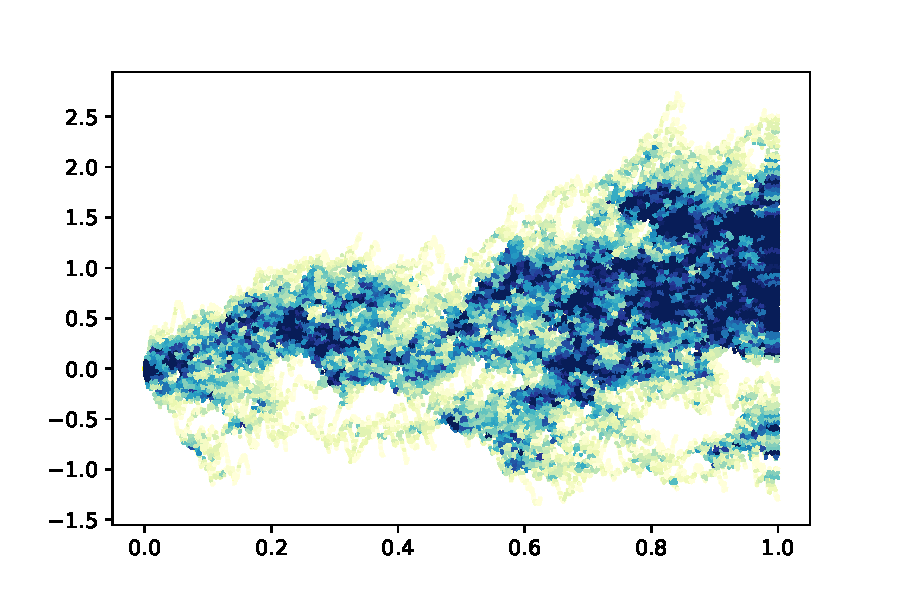
\includegraphics[scale= 0.7]{critical_Superprocess.pdf}
\end{figure}
\end{frame}

% ** Assumptions
\subsection{Assumptions}
% *** Assumptions for spatial motion
\begin{frame}{Model/Assumptions/Spatial motion}
  \begin{itemize}
  \item
    The mean semigroup of the superprocess:
    \[
      \mathbf P_{\delta_x} [X_t(f)] = {\color{red} P_t^\beta} f(x) := \Pi_x[e^{\int_0^{t} \beta (\xi_r) dr}f(\xi_t)].
    \]
  \end{itemize}
  \begin{block}{Assumption 1.}   
    There exist a $\sigma$-finite measure {\color{red} $m$} with full support on $E$ and a family of strictly positive,
    bounded continuous functions $\{ p_t(\cdot,\cdot): t > 0 \}$ on $E \times E$ such that
    \begin{itemize}
    \item $P_tf(x)= \int_E p_t(x,y) f(y) m(dy);$
    \item $\int_E p_t(y,x)m(dy) \leq 1;$
    \item $\int_E \int_E p_t(x,y)^2 m(dx) m(dy)
      <\infty;$
    \item
      $x \mapsto \int_E p_t(x,y)^2 m(dy)$ and $x \mapsto \int_E p_t(y,x)^2 m(dy)$ are both continuous.
    \end{itemize}
  \end{block}
\end{frame}

\begin{frame}{Model/Assumptions/Spatial motion}
  Under Assumption 1, we can say the following:
  \begin{itemize}
  \item
    $(P^\beta_t)_{t \geq 0}$ and its disjoint $(P^{\beta *}_t)_{t \geq 0}$ are strongly continuous semigroups of compact operators in $L^2(E,m)$.
  \item
    Let $L$ and $L^*$ be the generators of $(P^\beta_t)_{t \geq 0}$ and $(P^{\beta *}_t)_{t \geq 0}$, respectively. 
    Then ${\color{red} \lambda} := \sup \text{Re}(\sigma(L)) = \sup \text{Re}(\sigma(L^*))$ is a common {\color{red}eigenvalue} of multiplicity $1$ for both $L$ and $L^*$.
  \item
    The corresponding {\color{red}eigenfunctions} {\color{red} $\phi$} of $L$ and {\color{red} $\phi^*$} of $L^*$ can be chosen to be strictly positive and continuous everywhere on $E$.
  \item
    Normalize $\phi$ and $\phi^*$ by $\langle\phi, \phi\rangle_m = \langle\phi,\phi^*\rangle_m = 1$ so that they are unique.
  \item
    Operator $P_t^\beta$ has transition density {\color{red}$p_t^\beta(x,y)$} with respect to measure $m$.
  \end{itemize}
\end{frame}

% *** Assumptions for Mean semigroup and branching mechanism
\begin{frame}{Model/Assumptions/Mean semigroup and branching mechanism}
\begin{block}{Assumption 2. (Critical and Intrinsic Ultracontractive)}
\begin{itemize}
\item 
  $\lambda = 0$.
\item
  $\forall t > 0, \exists c_t>0, \forall x,y \in E, \quad p_t^\beta (x,y) \leq c_t \phi(x) \phi^*(y)$.
\end{itemize}
\end{block}
\begin{block}{Assumption 3 (Stable branching)}
  The branching mechanism $\psi$ is of the form:
  \begin{align*}
    \psi(x,z)
    = -\beta (x) z + \kappa(x) z^{\gamma(x)},
  \end{align*}
  where $\beta \in \mathscr B_b(E), \gamma \in \mathscr B^+_b(E)$, $\kappa \in \mathscr B^+_b(E)$ with $1< \gamma(\cdot )<2$. 
  We also assume that 
  \[{\color{red} \gamma_0} := \operatorname{ess\,inf}_{m(dx)} \gamma(x)> 1\] and $\kappa_0:=\operatorname{ess\,inf}_{m(dx)}\kappa(x) > 0$.
\end{block}
\end{frame}

% ** Slack type result
\subsection{Slack type results}
\begin{frame}{Results/Slack type results}
\begin{block}{Theorem 1}
Under Assumptions 1,2 and 4, we have
\begin{itemize}
\item[(1)]
  $\mathbf P_{\delta_x}( \| X_t\| = 0) > 0$, for each $t > 0$ and $x\in E$.
\item[(2)]
  For each $\mu \in \mathcal M$, $\mathbf P_{\mu}(\|X_t\| \neq 0) = {\color{red} t^{-\frac{1}{\gamma_0 - 1}}} L(t)$ where $L(t)$ is a slowly varing function at $\infty$.
\end{itemize}
Write $C_X := \langle \mathbf 1_{\gamma(\cdot) = {\color{red} \gamma_0}} \kappa\cdot \phi^{ \color{red} \gamma_0}, \phi^* \rangle_m$ and $\eta_t := \big( C_X(\gamma_0 - 1) {\color{red} t} \big)^{\color{red} - 1/(\gamma_0 - 1) }$. 
{\color{red} Further assume} that $m( x:\gamma(x)={\color{red}\gamma_0} )>0$, then
\begin{itemize}
\item[(3)]
$
  \lim_{t\to\infty} \eta_t^{-1}\mathbf P_{\mu}(\|X_t\| \neq 0)
  =\mu(\phi);
$
\item[(4)]
  for each $f \in \mathscr B^+(E)$ with $\langle f, \phi^* \rangle_m > 0$ and $\| \phi^{-1}f \|_\infty < \infty$,
\[
  \{\eta_t X_t(f) ; \mathbf P_{\mu}(\cdot |\|X_t\| \neq 0) \}
  \xrightarrow[t\to \infty]{d} \langle f, \phi^*\rangle_m {\color{red}\mathbf z^{(\gamma_0 - 1)}}.
\]
\end{itemize}
\end{block}
\end{frame}
% * Remarks
\section{Remarks}
\begin{frame}{Remarks/Slack type result}
  \begin{itemize}
  \item
    {\color{red} The asymptotic behavior} of the critical superprocesses with spatially dependent stable branching {\color{red} is dominated by the heaviest tail $\gamma_0$}.
  \item
    The weak limit is {\color{red} universal}: the distribution of $\mathbf z^{(\gamma_0 - 1)}$ is only related to $\gamma_0$.
  \item
    We proof the above results by characterizing some {\color{red} measure transform} of the superprocesses.
  \end{itemize}
  \begin{definition}[Size-biased transform]
    Let $G$ be a non-negative measurable function which is integrable with respect to a $\sigma$-finite measure $Q$.
    A probability measure {\color{red} $Q^G$} is called the $G$-transform of $Q$ if
    \[
      d{\color{red} Q^G} = \frac{G}{Q[G]} dQ.
    \]
  \end{definition}
\end{frame}
% * Methods
\section{Methods} 
% ** Size-biased transforms
\subsection{Size-biased transforms}
\begin{frame}{Methods: Size-biased add-on}
\begin{itemize}
\item Let $X$ be an non-negative r.v. with finite mean. Define
  \begin{align}
    {\color{red} F(\theta)}:= \frac{P^X[e^{-\theta X}]}{P[e^{-\theta X}]}, \quad \theta \geq 0.
  \end{align}
Then it holds that
\[
-\log \mathbf P[e^{-\theta X}] 
= \mathbf P[X] \int_0^\theta {\color{red} F(r)} dr
,\quad \theta \geq 0.
\]
\item
We call ${\color{red} F(\theta)}$ the {\color{red} size-biased add-on} function of the random variable $X$.
\item  
The distribution of $X$ is characterized by its mean and its size-biased add-on function.
\end{itemize}
\end{frame}

% ** Poisson random measures
\subsection{Poisson random measures}
\begin{frame}{Methods/Poisson random measures}
  \begin{block}{Lemma 1}
    Let $\mathcal N$ be a Poisson random measure with intensity measure $N$. 
    Let $F$ be a non-negative testing function with $0 < N[F] < \infty$.
    Then    
    \[
      \{\mathcal N; P^{\mathcal N(F)}\}
      \overset{d}{=} \{\mathcal N + {\color{red} \delta_s}; P \otimes {\color{red}N^F(ds)}\}.
    \]
  \end{block}
  \begin{figure}[h]
    \begin{tabular}{ll}
      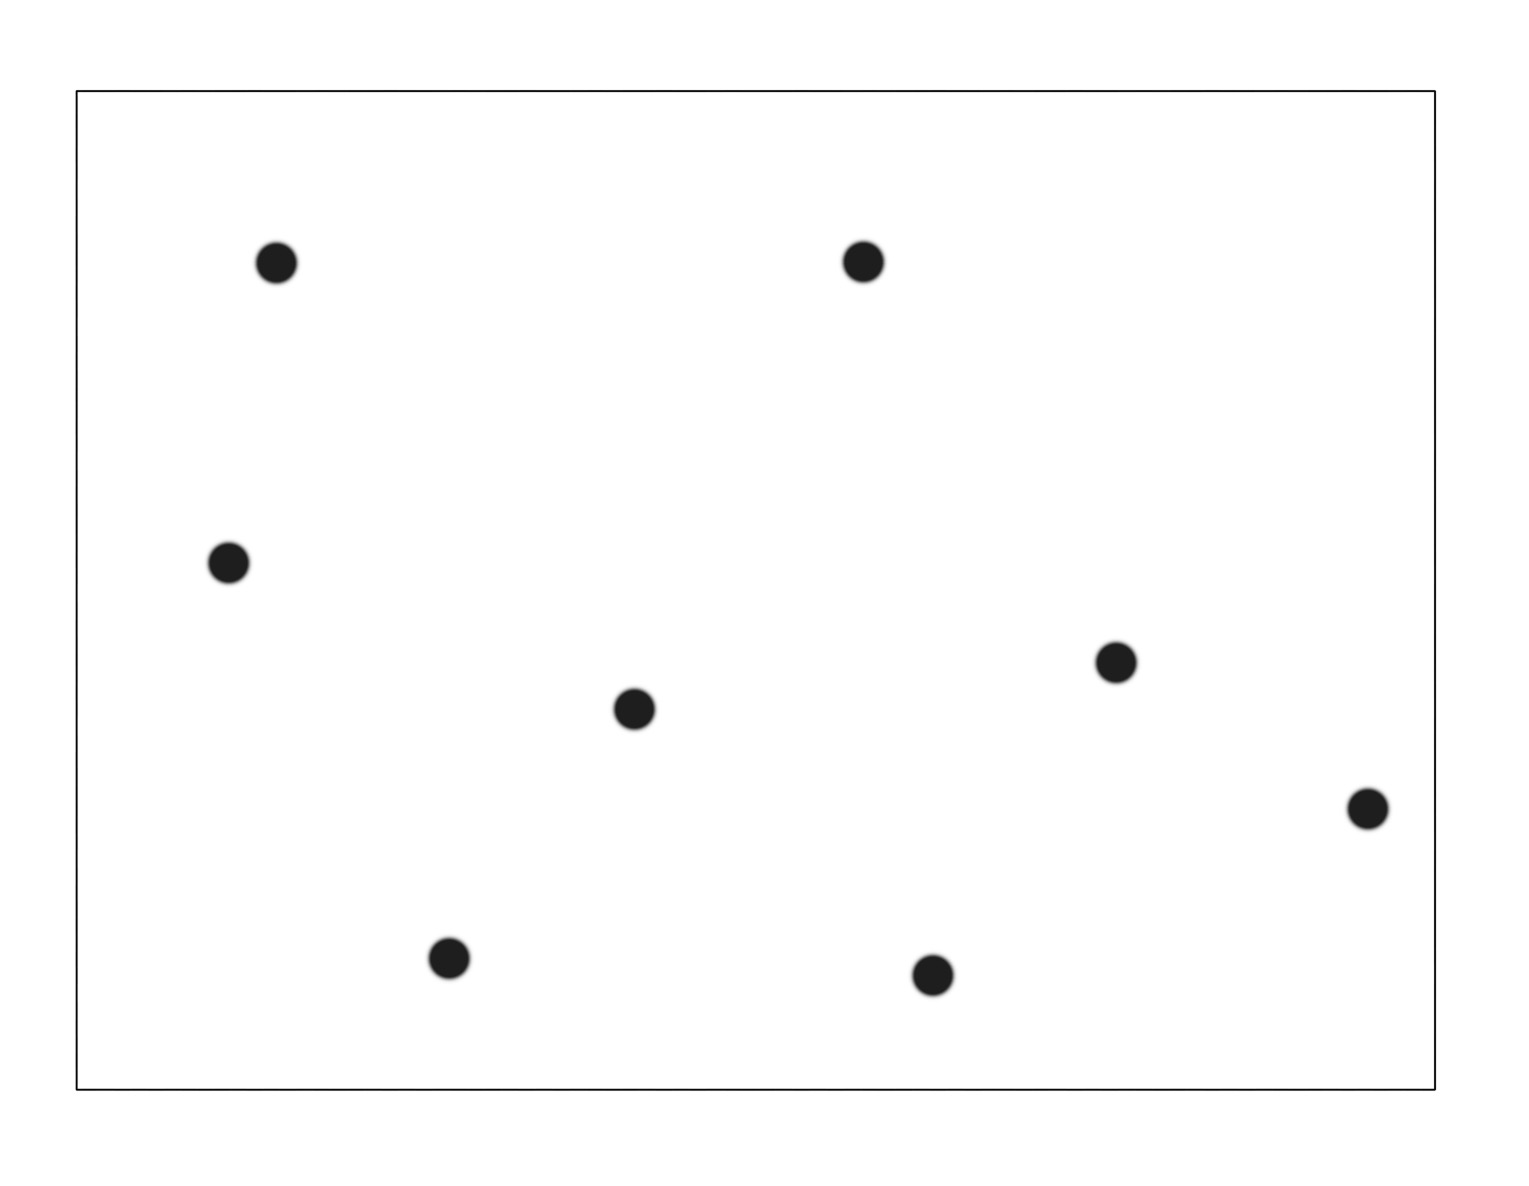
\includegraphics[scale=0.08]{001.jpg}
      &
        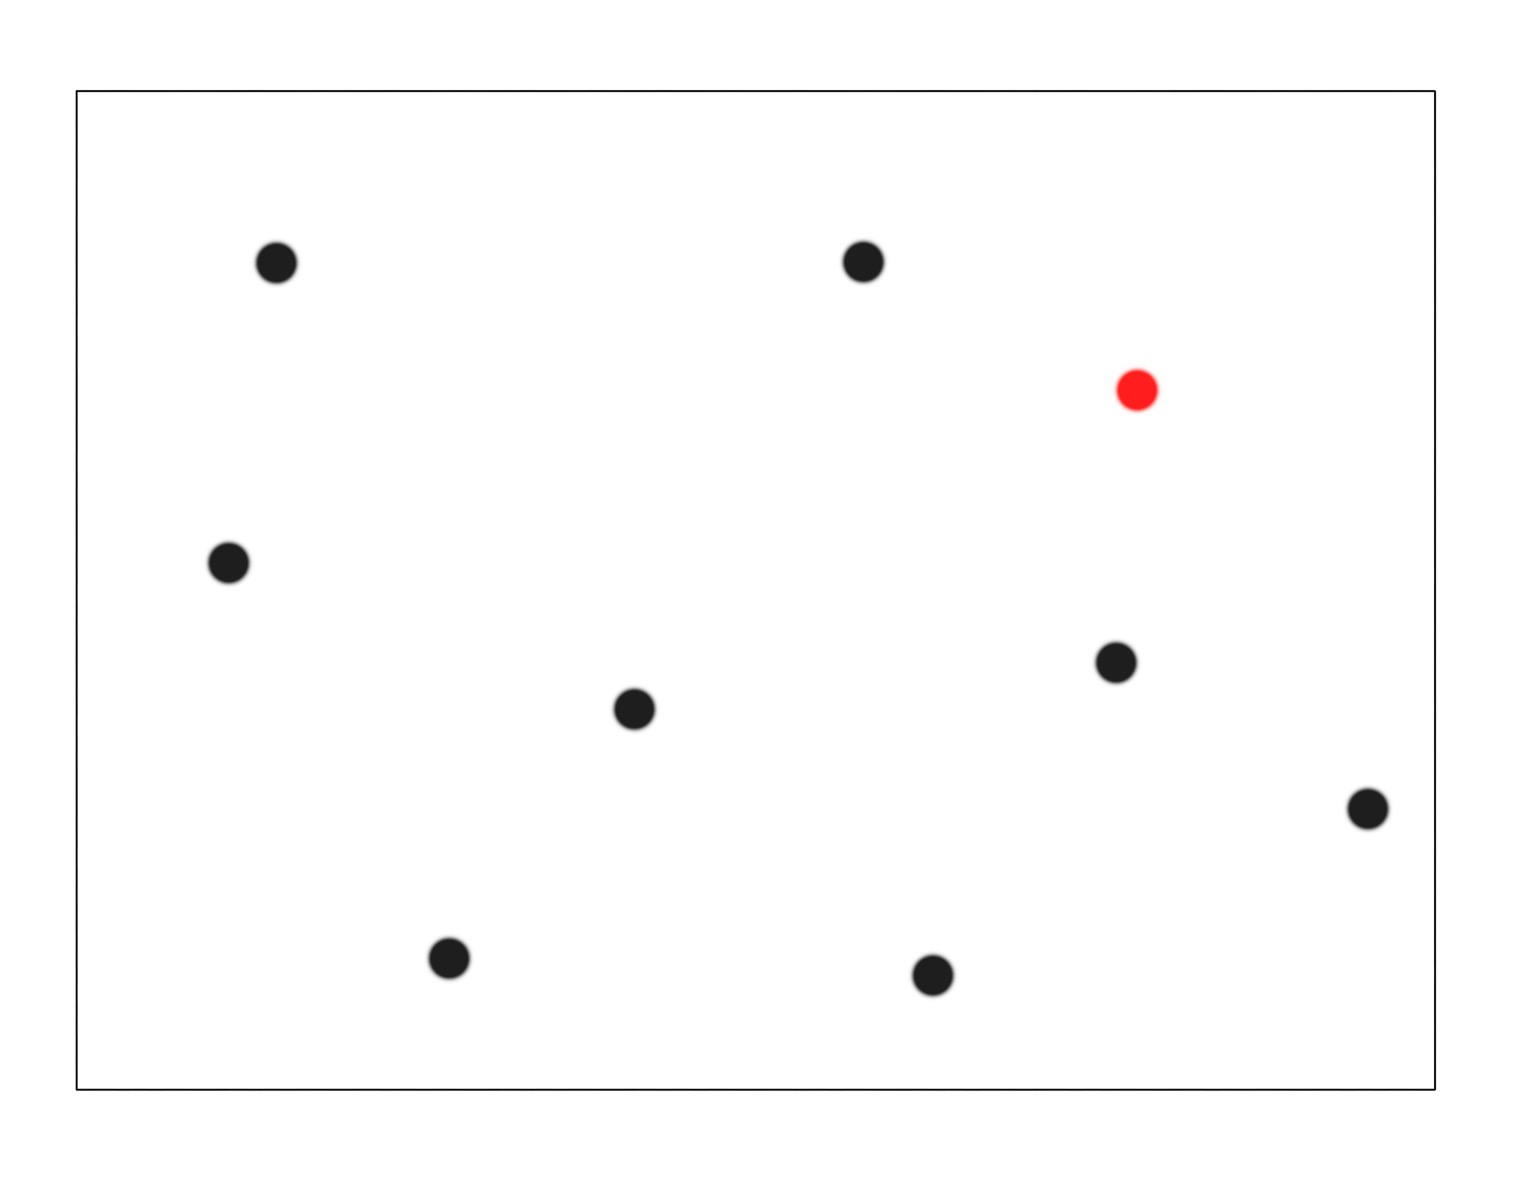
\includegraphics[scale=0.08]{002.jpg}
    \end{tabular}
  \end{figure}
\end{frame}

% ** Kuznetsov measures
\subsection{Kuznetsov measures}
\begin{frame}{Methods/Kuznetsov measures}
\begin{itemize}
\item
  The {\color{red} Kuznetsov measures $(\mathbb N_x)_{x\in E}$} of superprocess $(X_t)_{t\geq 0}$ is given by the following Theorem:
\end{itemize}
  \begin{theorem}[Li (2011) Theorem 8.24]
There is a family of $\sigma$-finite measures {\color{red} $(\mathbb N_x)_{x\in E}$} on space
\begin{align}
  \mathbb D &:= \{\mathcal M\text{-valued c\`adl\`ag functions on $[0,\infty)$} 
\\ &\qquad \text{with the null measure as a trap}\} 
\end{align}
such that for each $x\in E$, 
\begin{align}
\{(X_t)_{t>0}; \mathbf P_{\delta_x} \}
  \overset{d}{=} \left( \int_{\mathbb D} w_t \mathcal N(dw) \right)_{t>0},
\end{align}
where {\color{red} $\mathcal N$} is a Poisson random measure on $\mathbb D$ with intensity measure {\color{red} $\mathbb N_x$}.
\end{theorem}
\end{frame}

% ** Measure transform of superprocesses 
\subsection{Measure transform of superprocesses}
\begin{frame}{Methods/Measure transform of superprocesses}
\begin{block}{Theorem 3.}
  Let $\mu \in \mathcal M$ and write $\mathbb N_\mu(\cdot) := \int_{E} \mathbb N_x(\cdot)\mu(dx)$.
For each non-negative measurable function $F$ on $\mathbb D$ with $\mathbb N_\mu[F] \in (0,\infty)$, we have 
\begin{align}
\{(X_t)_{t\geq 0}; \mathbf P^{\mathcal N(F)}_\mu\} 
\overset{d}{=} \{(X_t)_{t\geq 0}; \mathbf P_\mu\} \otimes \{(w_t)_{t \geq 0}; \mathbb N^F_\mu(dw)\}.
\end{align}
\end{block}
    We can characterize $\{(w_t)_{t \geq 0}; \mathbb N^F_\mu(dw)\}$ while
    \begin{itemize}
    \item 
      $F(w) = w_t(\phi)$ using the {\color{red} classical Spine Decomposition Theorem}.
    \item 
      $F(w) = w_t(f)$ using a {\color{red} generalized Spine Decomposition Theorem}.
    \item 
      $F(w) = w_t(\phi)^2$ using a {\color{red} 2-Spine Decomposition Theorem.}
    \end{itemize}
\end{frame}
% ** Size-biased add-on functions
\subsection{Size-biased add-on functions}

\begin{frame}{Methods/Size-biased add-on functions}
Recall that
\begin{align}
- \log E[e^{\theta \mathbf z^{(\gamma_0 - 1)}}] 
  \approx 1 -  E[e^{\theta \mathbf z^{(\gamma_0 - 1)}}] 
= \left( \frac{1}{1+\theta^{-(\gamma_0- 1)}} \right)^{\frac{1}{\gamma_0 - 1}}
\end{align}
\begin{block}{Lemma 2}
The non-linear delay equation 
 \begin{align}
{\color{blue} G(\theta) } 
= \int_0^\theta {\color{red}\exp\left\{ - \frac{\gamma_0}{\gamma_0 - 1} \int_0^1  G(ru^{\frac{1}{\gamma_0 - 1}})^{\gamma_0 - 1} \frac{du}{u} \right\} } dr,
\quad \theta \geq 0,
  \end{align}
has a unique solution:
\begin{align}
G(\theta) 
  = \left( \frac{1}{1+\theta^{-(\gamma_0- 1)}} \right)^{\frac{1}{\gamma_0 - 1}},
\quad \theta \geq 0. 
\end{align}
\end{block}

So the {\color{red} red part} can be considered as an approximation of the size-biased add-on functions of random variable $\mathbf z^{(\gamma_0 - 1)}$.
\end{frame}

\begin{frame}{Methods/Size-biased add-on functions}
  Recall that ${\color{blue} V_T(\theta f)(x)} = - \log \mathbf P_{\delta_x}[e^{- \theta X_T(f)}]$
  \begin{block}{Theorem 4.}
    For each non-negative bounded measurable function $f$, each $\theta \geq 0, x\in E$ and $T > 0$, we have
    \begin{align}
      &{\color{blue}V_T(\theta f)(x)} 
      \\&= \phi(x) \int_0^\theta {\color{Red} \Pi_{x}^{(\phi)} \left[ \frac{f(\xi_T)}{\phi(\xi_T)} \exp \left\{ - \int_0^T \left( \kappa \gamma V_{T - s}(rf)^{\gamma - 1} (\xi_s) \right) \right\}\right] } dr.
    \end{align}
  \end{block}
\begin{itemize}
\item
  The {\color{red} red} part is the size-biased add-on function of $X_T(f)$.
\item  
From Theorem 4 and Lemma 2, we can verify (details omitted) that
  \begin{align}
    \frac{V_t(\theta \eta_t f)(x)}{\eta_t \phi(x)} 
    \xrightarrow[t\to \infty]{} G(\theta),\quad \theta >0.
  \end{align}
\end{itemize}
\end{frame}



% * Few References
\section{Few References}
\begin{frame}
\frametitle<presentation>{Few References}
    
\begin{thebibliography}{10} 
    
\beamertemplatearticlebibitems

\bibitem{RenSongSun2018Limit}
  Ren, Y.-X., Song, R. and Sun, Z.:
  \emph{Limit theorems for a class of critical superprocesses with stable branching.} ArXiv:1807.02837
  
  \bibitem{RenSongSun2017A-2-spine}
  Ren, Y.-X., Song, R. and Sun, Z.:
  \emph{A 2-spine decomposition of the critical Galton-Watson tree and a probabilistic proof of Yaglom's theorem.}
  Electron. Commun. Probab. 23 (2018), Paper No. 42, 12 pp.
 
  \bibitem{RenSongSun2017Spine}
  Ren, Y.-X., Song, R. and Sun, Z.:
  \emph{Spine decompositions and limit theorems for a class of critical superprocesses.}
  Acta Appl. Math. (2019), https://doi.org/10.1007/s10440-019-00243-7


  \end{thebibliography}
\end{frame}
\begin{frame}
  \centering \Large
  \emph{感谢!}
\end{frame}

\end{document}

%%% Local Variables: 
%%% TeX-engine: xetex
%%% End: